\documentclass[tikz,border=2mm]{standalone} 
\usetikzlibrary{positioning, decorations.text}

\begin{document}
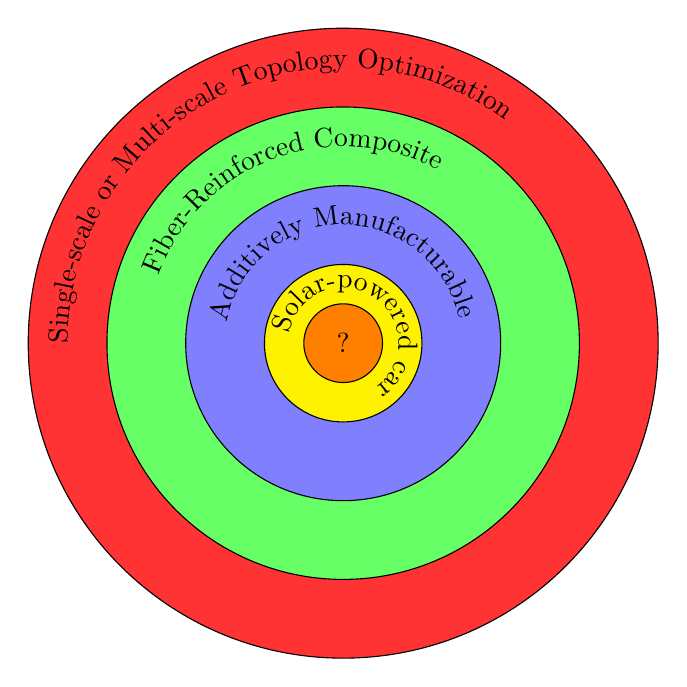
\begin{tikzpicture}

    \node[circle, minimum size=8cm, draw, fill=red!80] (a) {};
    \node[circle, minimum size=6cm, draw, fill=green!60] (b) {};
    \node[circle, minimum size=4cm, draw, fill=blue!50] (c) {};
    \node[circle, minimum size=2cm, draw, fill=yellow] (d) {};
    \node[circle, minimum size=1cm, draw, fill=orange] (e) {?};

    \draw [decorate, decoration={text along path, text = Single-scale or Multi-scale Topology Optimization}] (180:3.5) arc (180:0:3.5cm);

    \draw [decorate, decoration={text along path, text = Fiber-Reinforced Composite}] (160:2.5) arc (160:60:2.5cm);

    \draw [decorate, decoration={text along path, text = Additively Manufacturable}] (170:1.5) arc (170:-90:1.5cm);

    \draw [decorate, decoration={text along path, text = Solar-powered car}] (170:0.7) arc (170:-90:0.7cm);

\end{tikzpicture}
\end{document}